\emph{Authors: Marco Morandini and Riccardo Vescovini}
\newcommand{ \fracd }[ 2 ]{ \frac{ \displaystyle{ #1 } }{ \displaystyle{ #2 }} }
\newcommand{ \fracdp }[ 2 ]{ \frac{ \displaystyle{ \partial #1 } }{ \displaystyle{ \partial #2 }} }
\newcommand{ \Rot }[ 1 ]{ \texttt{Rot} \plbr{ #1 } }
\newcommand{ \VecRot }[ 1 ]{ \texttt{VecRot} \plbr{ #1 } }
\newcommand{ \valxii }[ 0 ]{\plbr{ \T{ \xi }_{ i } } }
\newcommand{ \valxin }[ 0 ]{\plbr{ \T{ \xi }_{ n } } }
\newcommand{ \valxiA }[ 0 ]{\plbr{ \T{ \xi }_{ A } } }
\newcommand{ \valxio }[ 0 ]{\plbr{ \T{ \xi }_{ 0 } } }
\noindent


%%%%%%%%%%%%%%%%%%%%%%%%%%%%%%
%%%%VARIATIONAL PRINCIPLE%%%%%
%%%%%%%%%%%%%%%%%%%%%%%%%%%%%%
\section{Variational principle}
The formulation refers to the modified Hu-Washizu variational functional. The linearization of the functional is written as:
\begin{equation}
\delta W + \Delta \delta W = 0
\end{equation}
with:
\begin{equation}
\delta W = \int_A \plbr{
\delta{\T{\epsilon}}^T \T{\sigma} + \delta \hat{\T{\epsilon}}^T \T{\sigma}
} \text{d}A
\label{eq:deltaW}
\end{equation}
with
\begin{align}
	\T{\sigma} &= \T{\sigma}\plbr{\T{\epsilon} + \hat{\T{\epsilon}}}
\end{align}
A linear (visco)elastic stress-strain relationship is considered,
\begin{align}
	\T{\sigma}
	&=
	\TT{C} \plbr{
		\T{\epsilon} + \hat{\T{\epsilon}}
	}
	+
	\TT{E} \plbr{
		\dot{\T{\epsilon}} + \dot{\hat{\T{\epsilon}}}
	}
\end{align}
\textbf{FIXME: $\dot{\hat{\T{\epsilon}}}$? Direi di no!}
and:
\begin{equation}
\Delta \delta W = \int_A \plbr{
\delta {\T{\epsilon}} ^T  \TT{C} \plbr{ \Delta {\T{\epsilon}}  + \Delta \hat{\T{\epsilon}}} +
\delta \hat{\T{\epsilon}} ^T  \TT{C} \plbr{ \Delta {\T{\epsilon}}  + \Delta \hat{\T{\epsilon}}} +
\Delta \delta { \T{\epsilon} }^T \T{\sigma}
} \text{d}A
\label{eq:DeltadeltaW}
\end{equation}
where:
\begin{itemize}
\item $\TT{C}$ and $\TT{E}$ are the linear viscoelastic constitutive law matrices (integrated along the shell thickness)
\item $\T{\epsilon}$ is the vector of the compatible strains (resulting from the strain-displacement relations)
\item $\T{\hat{\epsilon}}$ is the vector of the enhancing strains (EAS)
\item $\T{\sigma}$ is the vector of forces and moments per unit length
\end{itemize}
The enhancing strains $\T{\hat{\epsilon}}$ are interpolated within the element.\\
The compatible strains $\T{\epsilon}$ are defined as:
\begin{equation}
\underset{ 12 \times 1 }{
 \T{\epsilon}
 } =
\cubr{\vvect{c}{
 \tilde{\T{\epsilon}}_1 \\
 \tilde{\T{\epsilon}}_2 \\
 \tilde{\T{\kappa} }_1 \\
 \tilde{\T{\kappa} }_2 \\
}}
\end{equation}
where:
\begin{equation}
\tilde{\T{\epsilon}}_k =
\TT{T} ^T \T{y}_{,k}  - \T{e}_k
\label{eq:epsilon}
\end{equation}
where the comma followed by the index represents the derivation with respect to the $k$-th arc-length coordinate.\\
$\TT{T}$ is the orientation and $\T{y}$ is the position vector both in the deformed configuration, and $\T{e}_k=\{e_{1k},e_{2k},e_{3k}\}$, with
$e_{ik}=\delta_{ik}$.
\begin{equation}
\tilde{\T{\kappa}}_k  =
\TT{T}^ T \T{\kappa}_k  - \TT{T}_0 ^ T  \T{\kappa}^{0}_k
\end{equation}
with:
\begin{equation}
\T{\kappa}_k  \times = \TT{T}_{,k} \TT{T}^T
\end{equation}

\subsection{Strain Rate}
The compatible strain derivatives $\dot{\T{\epsilon}}$ are defined as:
\begin{equation}
\underset{ 12 \times 1 }{
 \dot{\T{\epsilon}}
 } =
\cubr{\vvect{c}{
 \dot{\tilde{\T{\epsilon}}}_1 \\
 \dot{\tilde{\T{\epsilon}}}_2 \\
 \dot{\tilde{\T{\kappa}}}_1 \\
 \dot{\tilde{\T{\kappa}}}_2 \\
}}
\end{equation}
where:
\begin{align}
	\frac{\mathrm{d}}{\mathrm{d}t} \tilde{\T{\epsilon}}_k
	&=
	\dot{\TT{T}}^T \T{y}_{,k}
	+
	\TT{T}^T \dot{\T{y}}_{,k}
	=
	-\TT{T}^T \T{\omega} \times \T{y}_{,k}
	+
	\TT{T}^T \dot{\T{y}}_{,k}
\end{align}
and
\begin{align}
	\frac{\mathrm{d}}{\mathrm{d}t} \tilde{\T{\kappa}}_k
	&=
	\dot{\TT{T}}^T \T{\kappa}_k
	+
	\TT{T}^T \dot{\T{\kappa}}_k
	=
	-\TT{T}^T \T{\omega} \times \T{\kappa}_k
	+
	\TT{T}^T \dot{\T{\kappa}}_k
	.
\end{align}
Since
\begin{align}
	\frac{\mathrm{d}}{\mathrm{d}t} (\TT{T}_{,k})
	&=
	\frac{\mathrm{d}}{\mathrm{d}t} (\T{\kappa}_k \times \TT{T})
	=
	\dot{\T{\kappa}}_k \times \TT{T}
	+
	\T{\kappa}_k \times \T{\omega} \times \TT{T}
	\\
	(\dot{\TT{T}})_{,k}
	&=
	(\T{\omega} \times \TT{T})_{,k}
	=
	\T{\omega}_{,k} \times \TT{T}
	+
	\T{\omega} \times \T{\kappa}_k \times \TT{T}
\end{align}
then
\begin{align}
	\dot{\T{\kappa}}_k \times + \T{\kappa}_k \times \T{\omega} \times 
	&=
	\T{\omega}_{,k} \times + \T{\omega} \times \T{\kappa}_k \times
\end{align}
i.e.\
\begin{align}
	\dot{\T{\kappa}}_k
	&=
	\T{\omega}_{,k}
	+
	\T{\omega} \times \T{\kappa}_k
\end{align}
Thus
\begin{align}
	\frac{\mathrm{d}}{\mathrm{d}t} \tilde{\T{\kappa}}_k
	&=
	\TT{T}^T \T{\omega}_{,k}
\end{align}

The vector $\T{\sigma}$ is:
\begin{equation}
 \T{\sigma} =
\cubr{\vvect{c}{
 \T{n}_1 \\
 \T{n}_2 \\
 \T{m}_1 \\
 \T{m}_2 \\
}}
\end{equation}
%%%%%%%%%%%%%%%%%%%%%%%%%%%%%%
%%%%%%%%NOTATION%%%%%%%%%%%%%%
%%%%%%%%%%%%%%%%%%%%%%%%%%%%%%
\section{Finite element discretization and notation}
The shell elements has four nodes, numbered counterclockwise
starting from the upper right node, as shown in Figure~\ref{fig:shell}.
\begin{figure}[htbp]
\centering
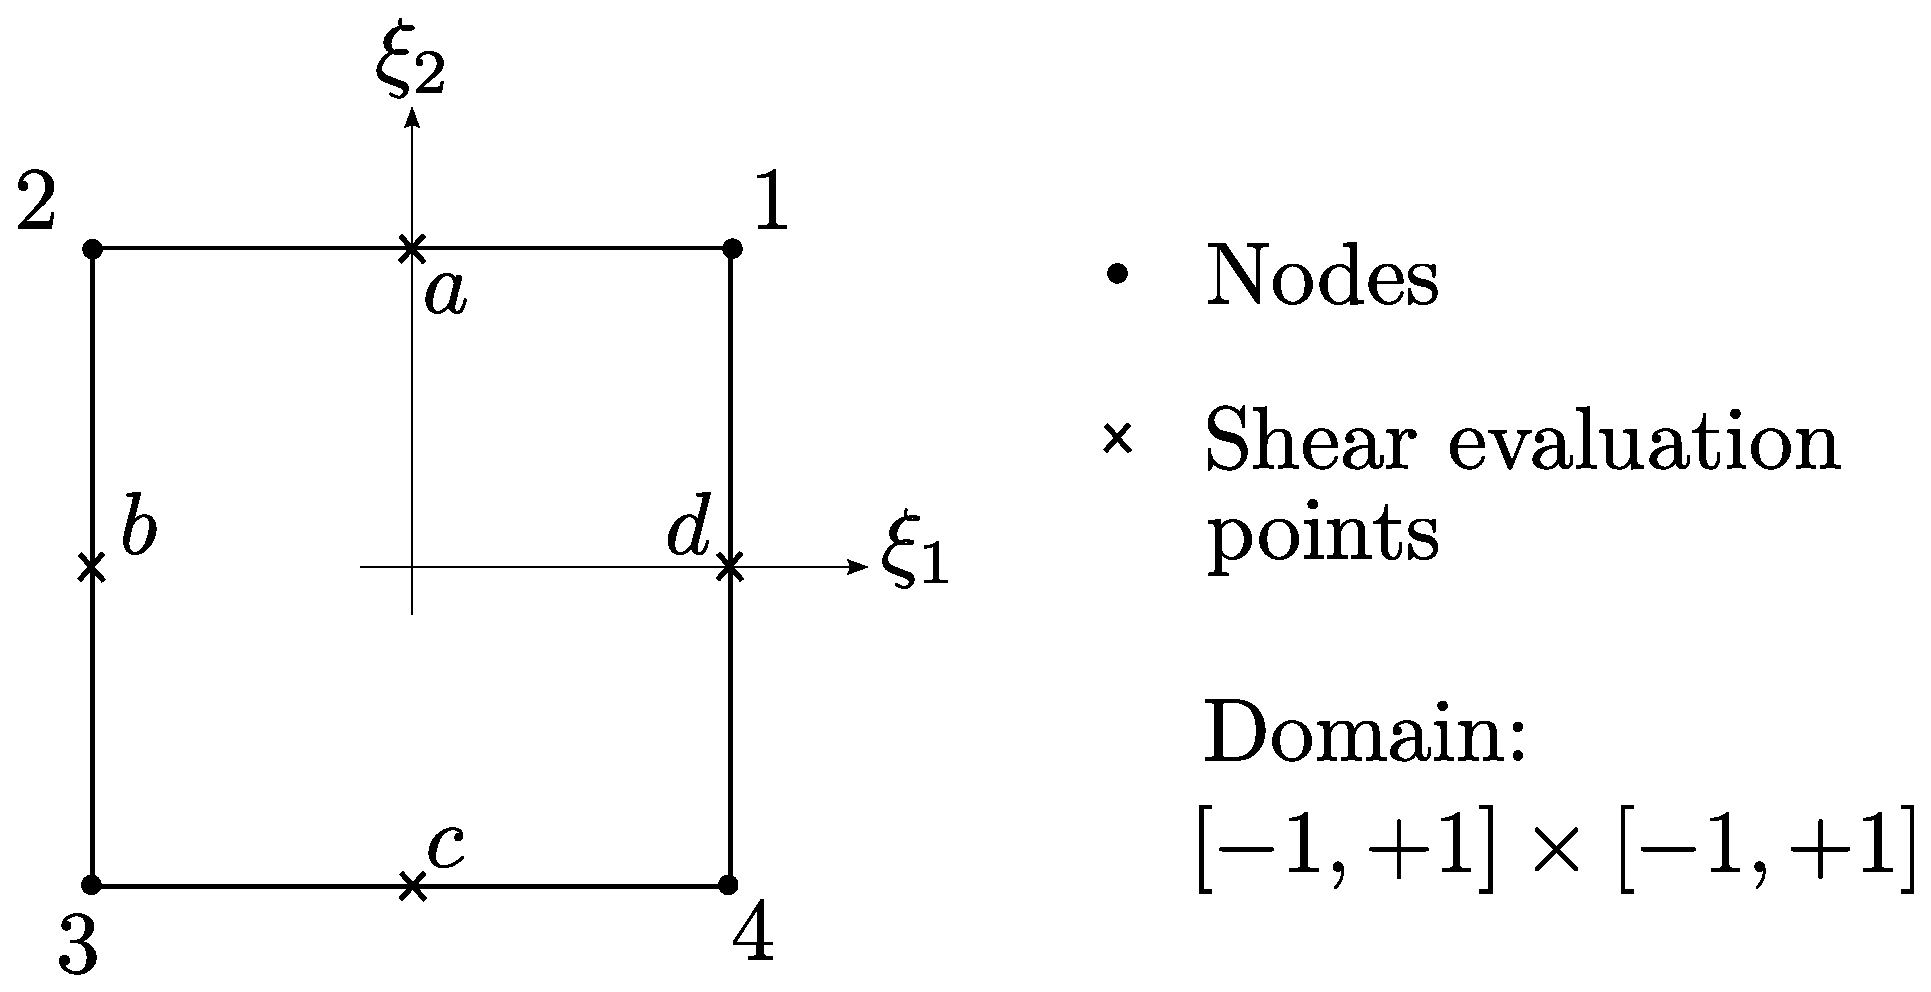
\includegraphics[width=8cm]{shellPic.eps}
\caption{Shell finite element}
\label{fig:shell}
\end{figure}
In the natural domain, the coordinate system is identified by the coordinates $\xi_1$ and $\xi_2$, both varying in the range $[-1, 1]$. \\
In the following, the notation
\begin{equation}
\T{\xi} = \plbr{\xi_{1},\xi_{2}}
\end{equation}
will be used.
Four points are defined at the element's mid-sides.
They are used in the context of the ANS approach.
In particular, they are denoted by the set of coordinates:
\begin{equation}
\vvect{c}{
\T{\xi}_a = \plbr{\xi_{1a},\xi_{2a}} \\
\T{\xi}_b = \plbr{\xi_{1b},\xi_{2b}} \\
\T{\xi}_c = \plbr{\xi_{1c},\xi_{2c}} \\
\T{\xi}_d = \plbr{\xi_{1d},\xi_{2d}}
}
\label{eq:xiSep}
\end{equation}
The following convention is adopted:
\begin{itemize}
	\item the subscript $n$ denotes a nodal variable
  \item $\T{\xi}_i$ means $\T{\xi}$ evaluated in a generic integration point
  \item $\T{\xi}_A$ means $\T{\xi}$ evaluated in one of the four shear evaluation points
  \item $\T{\xi}_0$ means $\T{\xi}$ evaluated at the origin
\end{itemize}
According to the numbering of the nodes, the bilinear shape functions defined at element level are:
\begin{subequations}
\begin{align}
L_1(\T{\xi}) & = \frac{1}{4} \plbr{ 1 + \xi_1 } \plbr{ 1 + \xi_2 } \\
L_2(\T{\xi}) & = \frac{1}{4} \plbr{ 1 - \xi_1 } \plbr{ 1 + \xi_2 } \\
L_3(\T{\xi}) & = \frac{1}{4} \plbr{ 1 - \xi_1 } \plbr{ 1 - \xi_2 } \\
L_4(\T{\xi}) & = \frac{1}{4} \plbr{ 1 + \xi_1 } \plbr{ 1 - \xi_2 }
\end{align}
\end{subequations}
The degrees of freedom associated to each element are 24 nodal position
and orientation parameter components, collected in vector ${\T{q}}$:
\begin{align}
\underset{24 \times 1}{\delta{\T{q}}}  =
\cubr{\vvect{c}{
\delta \T{y}_{n} \\
\T{\varphi}_{\delta n} \\
}}
 = &
\cubr{\vvect{c}{
\delta \T{y}_{1} \\
\T{\varphi}_{\delta 1} \\
\delta \T{y}_{2} \\
\T{\varphi}_{\delta 2} \\
\delta \T{y}_{3} \\
\T{\varphi}_{\delta 3} \\
\delta \T{y}_{4} \\
\T{\varphi}_{\delta 4} \\
}}
&
\underset{24 \times 1}{\Delta{\T{q}}}  =
\cubr{\vvect{c}{
\delta \T{y}_{n} \\
\T{\varphi}_{\Delta n} \\
}}
 = &
\cubr{\vvect{c}{
\Delta \T{y}_{1} \\
\T{\varphi}_{\Delta 1} \\
\Delta \T{y}_{2} \\
\T{\varphi}_{\Delta 2} \\
\Delta \T{y}_{3} \\
\T{\varphi}_{\Delta 3} \\
\Delta \T{y}_{4} \\
\T{\varphi}_{\Delta 4} \\
}}
\end{align}
and 7 internal degrees of freedom related to the assumed strain (EAS) and collected in vector $\T{\beta}$.\\
The total number of degrees of freedom is 31.
%%%%%%%%%%%%%%%%%%%%%%%%%%%%%%
%%%%%%%%%%LINEARIZATION%%%%%%%
%%%%%%%%%%%%%%%%%%%%%%%%%%%%%%
\section{Linearization}
The virtual variation of the compatible strains $\T{\epsilon}$ is
\begin{equation}
\delta \T{\epsilon} =
\cubr{\vvect{c}{
\delta \tilde{\T{\epsilon} }_1 \\
\delta \tilde{\T{\epsilon} }_2 \\
\delta \tilde{\T{\kappa} }_1 \\
\delta \tilde{\T{\kappa} }_2 \\
}}
\end{equation}
In particular, the virtual variations of the linear deformation $\tilde{\T{\epsilon} }_k $ is:
\begin{equation}
\delta \tilde{\T{\epsilon} }_k  = \delta \plbr{ \TT{T}^T \T{y}_{,k} } =
\sum_{i=1}^n \TT{T}^T \T{y}_{,k} \times \TT{\Phi}_{n} L_n \T{\varphi}_{\delta n} + \sum_{i=1}^n \TT{T}^T L_{n,k} \delta \T{y}_{n}
\label{eq:delta_epsilon}
\end{equation}
where:
\begin{equation}
\TT{\Phi}_{n} = \overline{\TT{T}}  \tilde{ \TT{\Gamma} } \tilde{ \TT{\Gamma} }_n^{-1} \overline{\TT{T}}^T
\end{equation}
The  virtual variations of the curvatures $\tilde{\T{\kappa} }_k$ is:
\begin{equation}
\delta \tilde{\T{\kappa} }_k = \delta \plbr{ \TT{T}^T \T{\kappa}_k } =
\sum_{i=1}^n \TT{T}^T \T{\kappa}_k \times \TT{\Phi}_n L_n \T{\varphi}_{\delta n} + \sum_{i=1}^n \TT{T}^T \TT{K}_{kn} \T{\varphi}_{\delta n}
\label{eq:delta_k}
\end{equation}
where:
\begin{equation}
\TT{K}_{kn} = \overline{\TT{T}} \mathcal{L} \plbr{ \tilde{\T{\varphi}}, \tilde{\T{\varphi}}_{,k} } \tilde{ \TT{\Gamma} }_{n}^{-1} \overline{T}^T L_n + \TT{\Phi}_{n} L_{n,k}
\end{equation}
the term $L_{n,k}$ is the derivative of the $n$-th shape function with respect to the $k$-th arc-length coordinate.\\
%%%%%%%delta delta%%%%%%%
The last term of Eq.~\ref{eq:DeltadeltaW} requires the evaluation of the terms:
\begin{equation}
\begin{split}
\T{n}_k \cdot \Delta \delta \tilde{\T{\epsilon}}_k =
\T{n}_k \cdot \Delta \delta \plbr{ \TT{T}^T \T{y}_{,k} } & =
\sum_{m,n=1}^{4} \T{\varphi}_{\delta n} \TT{\Phi}_{n}^T L_n \T{y}_{,k} \times \plbr{ \TT{T} \T{n}_k } \times \TT{\Phi}_m L_m  \T{\varphi}_{\Delta n} + \\
& + \sum_{m,n=1}^{4} \T{\varphi}_{\delta n} \TT{\Phi}_{n}^T L_n \plbr{\TT{T} \T{n}_k} \times L_{m,k} \Delta \T{y}_{n} + \\
& - \sum_{m,n=1}^{4} \delta \T{y}_n L_{n,k} \plbr{\TT{T} \T{n}_k} \times \TT{\Phi}_m L_m \T{\varphi}_{\Delta m}
\end{split}
\label{eq:Deltadelta_epsilon}
\end{equation}
\begin{equation}
\begin{split}
\T{m}_k \cdot \Delta \delta \tilde{\T{\kappa}}_k =
\T{m}_k \cdot \Delta \delta \plbr{\TT{T}^T \T{\kappa}_k} & =
\sum_{m,n=1}^{4} \T{\varphi}_{\delta n} L_n \TT{\Phi}_n^T \T{\kappa}_k \times \plbr{\TT{T} \T{m}_k} \times \T{\Phi_{m}} L_m \T{\varphi}_{\Delta m} + \\
&+\sum_{m,n=1}^{4} \T{\varphi}_{\delta n} L_n \TT{\Phi}_n^T \plbr{\TT{T} \T{m}_k} \times \TT{\Phi}_m L_{m,k} \T{\varphi}_{\Delta m}
\end{split}
\label{eq:Deltadelta_k}
\end{equation}
%%%%%%%%%%%%%%%%%%%%%%%%%%%%%%
%%%%%%%%%STRUCTURAL DAMPING%%%
%%%%%%%%%%%%%%%%%%%%%%%%%%%%%%
\section{Structural Damping}
Consistently formulated structural damping requires to express
the time derivatives of strain and curvature.
A linear contribution to internal force and moment fluxes is considered,
\begin{align}
	\T{\sigma}
	& \text{ += }
	\TT{E} \dot{\T{\epsilon}}
\end{align}
The discretized strain rate is
\begin{align}
	\frac{\mathrm{d}}{\mathrm{d}t} \tilde{\T{\epsilon}}_k
	&=
	\TT{T}^T \T{y}_{,k} \times \sum_{i=1}^n \TT{\Phi}_i L_i \T{\omega}_i
	+
	\TT{T}^T \sum_{i=1}^n L_{n,k} \dot{\T{y}}_i
\end{align}
The discretized curvature rate is
\begin{align}
	\frac{\mathrm{d}}{\mathrm{d}t} \tilde{\T{\kappa}}_k
	&=
	\TT{T}^T \sum_{i=1}^n L_{n,k} \T{\omega}_i
\end{align}

%%%%%%%%%%%%%%%%%%%%%%%%%%%%%%
%%%%%%%%%IMPLEMENTATION%%%%%%%
%%%%%%%%%%%%%%%%%%%%%%%%%%%%%%
\section{Implementation}
Having shown the variational principle and the linearization of strains and curvatures, it is then possible to develop the procedure to derive the Jacobian matrix and the residual.
%%%%%%%%%%%%%%%%%%%%%%%%%%%%%%
%%%%%%%%%%%ORIENTATION%%%%%%%%
%%%%%%%%%%%%%%%%%%%%%%%%%%%%%%
\subsection{Orientation interpolation}
In the initial configuration it is built the matrix:
\begin{equation}
\T{ iTa }_n = \TT{R}_n^T \sqbr{ \T{ t }_{ 1n } \T{ t }_{ 2n } \T{ t }_{ 3n } }
\end{equation}
with $\TT{R}_n$ node orientation, and $\T{t}_{in}$ vectors tangent to the element surface.\\
So:
\begin{equation}
\TT{T}_{n} = \TT{R}_n \T{ iTa }_n
\end{equation}
It is then calculated:
\begin{equation}
\TT{T}_\text{avg} = \fracd{ 1 }{ 4 } \sum_{ n = 1 }^{ 4 } \TT{T}_n
\end{equation}
which is in general a not orthogonal matrix.\\
An orthogonal matrix can be obtained by applying:
\begin{equation}
\overline{ \TT{T} } = \Rot{ \VecRot{ \TT{T}_\text{avg} }  }
\end{equation}
which is then used to calculate the nodal rotation:
\begin{equation}
\tilde{ \TT{R} }_{ n } = \overline{ \TT{T} } ^T \TT{T}_n
\end{equation}
and:
\begin{equation}
\tilde{ \T{\varphi} }_n = \VecRot{ \tilde{ \TT{R} }_n }
\end{equation}
The nodal values of $\tilde{ \T{\varphi} }_n$ are interpolated by means of the shape functions:
\begin{equation}
\tilde{ \T{ \varphi } } \valxii = \sum_{ i = 1 }^{ 4 } L_n \valxii \tilde{ \T{ \varphi } }_n
\end{equation}
from which is obtained the rotation matrix at the integration point:
\begin{equation}
\tilde{ \TT{R} } \valxii = \Rot{ \tilde{ \T{\varphi} } \valxii }
\end{equation}
and finally the orientation at the integration point:
\begin{equation}
\TT{T} \valxii = \overline{ \TT{T} } \tilde{ \TT{R} } \valxii
\end{equation}
The virtual variation of $\T{\varphi}$ at the integration point is related to the nodal values by:
\begin{equation}
\T{ \varphi }_{\delta} \valxii =
\sum_{ n = 1 }^{ 4 } \T{ \Phi }_n \valxii L_n \valxii \T{\varphi}_{\delta n}
\end{equation}
with:
\begin{equation}
\T{ \Phi }_n \valxii =
\overline{ \TT{T} } \tilde{\TT{\Gamma}} \plbr{ \tilde{ \T{\varphi}}  \valxii }  \tilde{\TT{\Gamma}} ^ {-1} \plbr{ \tilde{ \T{\varphi} }_n } \overline{ \TT{T} } ^ T
\end{equation}
Similarly the virtual variation of $\T{\varphi}$ can be obtained at the shear evaluation points as:
\begin{equation}
\T{ \varphi }_{\delta} \valxiA =
\sum_{ n = 1 }^{ 4 } \T{ \Phi }_n \valxiA L_n \valxiA \T{\varphi}_{\delta n}
\end{equation}
%%%%%%%%%%%%%%%%%%%%%%%%%%%%%%
%%%%%%%%%%%POSITION%%%%%%%%%%%
%%%%%%%%%%%%%%%%%%%%%%%%%%%%%%
\subsection{Position interpolation}
The nodal positions are so interpolated as:
\begin{equation}
\T{ y }   = \sum_{ n = 1 }^4  L_n   \T{ y }_n
\end{equation}
The derivatives with respect to the generic coordinate $\xi_k$ at the integration points is:
\begin{equation}
\fracdp{ \T{ x } \valxii }{ \xi_k }  = \sum_{ n = 1 }^4 \fracdp{ L_n \valxii }{ \xi_k } \T{ x }_n
\end{equation}
It is then possible to build the matrix:
\begin{equation}
\underset{ 2 \times 2 }{ \TT{S}_{ \alpha \beta } \valxii } =
\sqbr{ \matr{ c  c  }{
\underset{ 1 \times 3 }{ \T{ t }_{1}^{0} \valxii } \underset{ 3 \times 1 }{ \fracdp{ \T{x} \valxii }{ \xi_1 } } & \T{ t }_{1}^{0} \valxii \fracdp{ \T{x} \valxii }{ \xi_2 } \\
\T{ t }_{2}^{0} \valxii \fracdp{ \T{x} \valxii }{ \xi_1 } & \T{ t }_{2}^{0} \valxii \fracdp{ \T{x} \valxii }{ \xi_2 }
}}
\end{equation}
observing that $\TT{T}_0 \valxii = \sqbr{ \T{t}_{1}^{0} \valxii  \T{t}_{2}^{0} \valxii \T{t}_{3}^{0} \valxii }$.\\
With the same procedure are derived $\TT{S}_{ \alpha \beta } \valxio$ and  $\TT{S}_{ \alpha \beta } \valxiA$.\\
\begin{equation}
\underset{ 4 \times 2 } { \TT{L}_{ \alpha B } \valxii } =
\sqbr{ \matr{ c c }{
\fracdp{ L_1 \valxii }{ \xi_1 } & \fracdp{ L_1 \valxii }{ \xi_2 } \\
\fracdp{ L_2 \valxii }{ \xi_1 } & \fracdp{ L_2 \valxii }{ \xi_2 } \\
\fracdp{ L_3 \valxii }{ \xi_1 } & \fracdp{ L_3 \valxii }{ \xi_2 } \\
\fracdp{ L_4 \valxii }{ \xi_1 } & \fracdp{ L_4 \valxii }{ \xi_2 } \\
}}
\end{equation}
\begin{equation}
\underset{ 4 \times 2 } { \TT{L}_{ \alpha \beta } \valxii }=
\TT{L}_{ \alpha B } \valxii \TT{S}_{\alpha \beta} ^{-1} \valxii
\end{equation}
which is the matrix giving the variation of the shape functions $L_n$ with respect the the arc-length coordinates:
\begin{equation}
\TT{L}_{\alpha \beta} =
\sqbr{ \matr{ c c }{
L_{1,1} & L_{1,2} \\
L_{2,1} & L_{2,2} \\
L_{3,1} & L_{3,2} \\
L_{4,1} & L_{4,2}
}}
\end{equation}
In order to perform the integration in the isoparametric domain the area element need to be calculated. In particular, the determinant of the Jacobian of the transformation between the physical and the natural domain has to be calculated. It is:
\begin{align}
\alpha \valxii & = \det \TT{S}_{\alpha \beta} \valxii &
\alpha \valxiA & = \det \TT{S}_{\alpha \beta} \valxiA
\end{align}
%%%%%%%%%%%%%%%%%%%%%%%%%%%%%%
%%%%%%%%%%%%EAS%%%%%%%%%%%%%%%
%%%%%%%%%%%%%%%%%%%%%%%%%%%%%%
\subsection{Enhancing strains interpolation}
The virtual variation and increments of the enhancing strains $\T{\hat{\epsilon}}$ are interpolated as:
\begin{align}
\underset{12 \times 1}{\delta \hat{\T{\epsilon}}} \valxii & = \underset{12 \times 7}{\TT{P}} \valxii \underset{7 \times 1}{ \delta \T{\beta}} &  \Delta \hat{\T{\epsilon}}\valxii & = \TT{P}\valxii \Delta \T{\beta}
\end{align}
where $\T{\beta}$ is the vector collecting the the strains parameters, while the expression of the matrix $\TT{P}$ is derived in the next. \\
The EAS approach here adopted considers the enhancing of the membrane strains only, i.e. $\epsilon_{11}$, $\epsilon_{12}$, $\epsilon_{21}$ and $\epsilon_{22}$. Shear strains and bending strains are not enhanced.\\
The interpolation is performed in the natural domain adopting the shape functions:
\begin{equation}
\underset{ 4 \times 7 } { \TT{H} \valxii } =
\sqbr{ \matr{ c c c c c c c }{
\xi_{1i} & \xi_{1i} \xi_{2i} &  0    &      0      &   0   &      0      &   0     \\
  0   &      0      & \xi_{2i} & \xi_{1i} \xi_{2i} &   0   &      0      &   0     \\
  0   &      0      &  0    &      0      & \xi_{1i} & \xi_{1i} \xi_{2i} &   0      \\
  0   &      0      &  0    &      0      &   0   & \xi_{1i} \xi_{2i} & \xi_{2i}
}}
\end{equation}
The interpolation is reported in the physical domain with a push-forward operation with the transformation matrix $\TT{M}_0$, defined as:
\begin{equation}
\underset{ 4 \times 4 } { \TT{M}_0 } =
\sqbr{ \matr{ c c c c}{
s_{ 1, 1 } s_{ 1, 1 } & s_{ 1, 2 } s_{ 1, 2 } & s_{ 1, 2 } s_{ 1, 1 } &  s_{ 1, 1 } s_{ 1, 2 } \\
s_{ 2, 1 } s_{ 2, 1 } & s_{ 2, 2 } s_{ 2, 2 } & s_{ 2, 2 } s_{ 2, 1 } &  s_{ 2, 1 } s_{ 2, 2 } \\
s_{ 1, 1 } s_{ 2, 1 } & s_{ 1, 2 } s_{ 2, 2 } & s_{ 1, 1 } s_{ 2, 2 } &  s_{ 1, 2 } s_{ 2, 1 } \\
s_{ 1, 1 } s_{ 2, 1 } & s_{ 1, 2 } s_{ 2, 2 } & s_{ 1, 2 } s_{ 2, 1 } &  s_{ 1, 1 } s_{ 2, 2 }
}}
\end{equation}
where the generic term $s_{ i, k }$ is the element $\plbr{i,k}$ of the matrix $\TT{S}_{ \alpha \beta } \valxio$.\\
\begin{equation}
\underset{ 12 \times 7 }{ \TT{P} \valxii } =
\fracd{ \alpha \valxio }{ \alpha \valxii } \underset{ 12 \times 4  }{ \T{\mathcal{P}} } \underset{ 4 \times 4 }{ \TT{M}_{0}^{-T} } \underset{ 4 \times 7 }{ \TT{H} \valxii }
\end{equation}
where $\T{\mathcal{P}}$ is a permutation matrix defined as:
\begin{equation}
\underset{ 12 \times 4 }{ \T{\mathcal{P}} } =
\sqbr{ \matr{ c c c c  }{
1 & 0 & 0 & 0 \\
0 & 0 & 1 & 0 \\
0 & 0 & 0 & 0 \\
0 & 0 & 0 & 1 \\
0 & 1 & 0 & 0 \\
0 & 0 & 0 & 0 \\
0 & 0 & 0 & 0 \\
0 & 0 & 0 & 0 \\
0 & 0 & 0 & 0 \\
0 & 0 & 0 & 0 \\
0 & 0 & 0 & 0 \\
0 & 0 & 0 & 0
}}
\end{equation}
which has the places the enhanced strains in the corresponding positions of the global vector of membrane and bending strains $\T{\epsilon}$.
%%%%%%%%%%%%%%%%%%%%%%%%%%%%%%
%%%%%COMAPTIBLE STRAINS%%%%%%
%%%%%%%%%%%%%%%%%%%%%%%%%%%%%%
\subsection{Compatible strains interpolation}
The virtual variations of the linear deformation $\tilde{\T{\epsilon} }_k $ at the $i$-th integration point is obtained from Eq.~\ref{eq:delta_epsilon}:
\begin{equation}
\begin{split}
\delta \tilde{\T{\epsilon} }_k \valxii & = \delta \plbr{ \TT{T}\valxii^T \T{y}_{,k} \valxii } = \\
& \sum_{i=1}^n \TT{T}\valxii^T \T{y}_{,k}\valxii \times \TT{\Phi}_{n} \valxii L_n \valxii \T{\varphi}_{n \delta} + \sum_{i=1}^n \TT{T}\valxii^T \TT{L}_{\alpha \beta} \valxii \plbr{ n, k } \valxii \delta \T{y}_{n}
\end{split}
\label{eq:delta_epsilon_i}
\end{equation}
where $\TT{L}_{\alpha \beta} \valxii \plbr{ n, k }$ denotes the element $\plbr{n, k}$ of the matrix $\TT{L}_{\alpha \beta} \valxii$.\\
The  virtual variation of the curvatures $\tilde{\T{\kappa} }_k$ at the $i$-th integration point is derived from Eq.~\ref{eq:delta_k}:
\begin{equation}
\begin{split}
\delta \tilde{\T{\kappa} }_k \valxii & = \delta \plbr{ \TT{T}\valxii^T \T{\kappa}_k \valxii} =  \\
& \sum_{i=1}^n \TT{T}\valxii^T \T{\kappa}_k\valxii \times \TT{\Phi}_n\valxii L_n\valxii \T{\varphi}_{n \delta} + \sum_{i=1}^n \TT{T}\valxii^T \TT{K}_{kn}\valxii \T{\varphi}_{n \delta}
\end{split}
\label{eq:delta_k_i}
\end{equation}
where:
\begin{equation}
\TT{\Phi}_{n} \valxii = \overline{\TT{T}}  \tilde{ \TT{\Gamma} } \plbr{ \tilde{\T{\varphi}} \valxii } \tilde{ \TT{\Gamma} }_n^{-1} \overline{\TT{T}}^T
\end{equation}
and:
\begin{equation}
\TT{K}_{kn} \valxii =
\overline{\TT{T}} \mathcal{L} \plbr{ \tilde{\T{\varphi}}\valxii, \tilde{\T{\varphi}}_{,k}\valxii } \tilde{ \TT{\Gamma} }_{n}^{-1} \overline{T}^T L_n\valxii + \TT{\Phi}_{n}\valxii \TT{L}_{\alpha \beta} \valxii \plbr{ n, k } \valxii
\end{equation}
The derivative of the the vector $\tilde{\T{\varphi}}$ with respect to the $k$-th arc-length coordinate can be expressed as function of the nodal values as:
\begin{equation}
\tilde{ \T{ \varphi } }_{,k} \valxii  =
\sum_{n=1}^4 \TT{L}_{\alpha \beta} \valxii \plbr{ n, k } \T{\varphi}_{n}
\end{equation}
The curvatures are given by:
\begin{equation}
\T{\kappa}_k \valxii  =
\overline{\TT{T}} \tilde{\TT{\Gamma}} \plbr{ \tilde{\T{\varphi}} \valxii } \tilde{ \T{\varphi} }_{,k} \valxii
\end{equation}
and the derivative of the position vector is:
\begin{equation}
\T{y}_{,k} \valxii  =
\sum_{i=1}^{4} \TT{L}_{\alpha \beta} \valxii \plbr{n,k} \T{y}_n
\end{equation}
The compatible strains can so be expressed as function of the nodal variables $\T{q}$ by considering Eqs.~\ref{eq:delta_epsilon_i} and \ref{eq:delta_k_i}:
\begin{equation}
\delta \T{\epsilon} = \overline{\TT{B}} \delta{\T{q}}
\end{equation}
with:
\begin{equation}
\underset{ 12 \times 24 }{\overline{\TT{B}} \valxii} =
\sqbr{ \matr{ c c c c  }{
\overline{\TT{B}}_1 \valxii & \overline{\TT{B}}_2 \valxii & \overline{\TT{B}}_3 \valxii & \overline{\TT{B}}_4 \valxii
}}
\label{eq:B_overline}
\end{equation}
and:
\begin{equation}
\underset{ 12 \times 6 }{\overline{\TT{B}}_n \valxii} =
\sqbr{ \matr{ c c  }{
\TT{T} \valxii^T \TT{L}_{\alpha \beta} \valxii \plbr{n,1} & \TT{T}\valxii^T \T{y}_{,1} \valxii \times \TT{\Phi}_{n} \valxii L_{n} \valxii \\
\TT{T} \valxii^T \TT{L}_{\alpha \beta} \valxii \plbr{n,2} & \TT{T}\valxii^T \T{y}_{,2} \valxii \times \TT{\Phi}_{n} \valxii L_{n} \valxii \\
0 & \TT{T}\valxii^T \T{\kappa}_{1} \valxii \times \TT{\Phi}_{n} \valxii L_{n} \valxii + \TT{T} \valxii^T \TT{K}_{1n} \valxii \\
0 & \TT{T}\valxii^T \T{\kappa}_{2} \valxii \times \TT{\Phi}_{n} \valxii L_{n} \valxii + \TT{T} \valxii^T \TT{K}_{2n} \valxii
}}
\end{equation}
%%%%%%%%%%%%%%%%%%%%%%%%%%%%%%
%%%%%%%%%%ANS%%%%%%%%%%%%%%%%%
%%%%%%%%%%%%%%%%%%%%%%%%%%%%%%
\subsection{ANS}
The ANS technique is applied to prevent shear locking. Here the ANS is applied to shear strains only, i.e. $\epsilon_{1}$ and  $\epsilon_{2}$ The approach consists in interpolating the shear strains in the mid-sides of the element in the natural domain. Such interpolated strains are then used to derive the shear strains at the integration points.\\
The use of the ANS technique leads a re-definition of:
\begin{itemize}
	\item the two rows of the $\overline{\TT{B}}$ matrix relative to shear strains
	\item the shear strains
\end{itemize}
The compatible strains are:
\begin{align}
\tilde{\T{\epsilon}}_1 & =
\cubr{\vvect{c}{
\epsilon_{11} \\
\epsilon_{12} \\
\epsilon_{1}
}}
&
\tilde{\T{\epsilon}}_2 & =
\cubr{\vvect{c}{
\epsilon_{21} \\
\epsilon_{22} \\
\epsilon_{2}
}}
\end{align}
At first, the compatible strains are evaluated at the shear evaluation points of Figure~\ref{fig:shell}. This is done referring to Eq.~\ref{eq:epsilon}
\begin{equation}
\tilde{\T{\epsilon}}_k \valxiA  =
\TT{T} \valxiA ^T \T{y}_{,k} \valxiA - \T{e}_k
\end{equation}
The matrix $\overline{\TT{B}}$ of Eq.~\ref{eq:B_overline} is built also in the shear evaluation points for the membrane strains only, and is indicated as $\overline{\overline{\TT{B}}}$
\begin{equation}
\underset{ 6 \times 24 }{\overline{\overline{\TT{B}}} \valxiA} =
\sqbr{ \matr{ c c c c  }{
\overline{\overline{\TT{B}}}_1 \valxiA & \overline{\overline{\TT{B}}}_2 \valxiA & \overline{\overline{\TT{B}}}_3 \valxiA & \overline{\overline{\TT{B}}}_4 \valxiA
}}
\end{equation}
with:
\begin{equation}
\underset{ 6 \times 6 }{\overline{\overline{\TT{B}}}_n \valxiA} =
\sqbr{ \matr{ c c  }{
\TT{T} \valxiA ^ T \TT{L}_{\alpha \beta} \valxiA \plbr{n,1} & \TT{T} \valxiA^T \T{y}_{,1} \valxiA \times \TT{\Phi}_{n} \valxiA L_{n}  \valxiA \\
\TT{T} \valxiA ^ T \TT{L}_{\alpha \beta} \valxiA \plbr{n,2} & \TT{T} \valxiA^T \T{y}_{,2} \valxiA \times \TT{\Phi}_{n} \valxiA L_{n}  \valxiA
}}
\end{equation}
The rows relative to the shear strains $\epsilon_1$ and $\epsilon_2$ are collected in:
\begin{align}
\underset{ 4 \times 24 }{\overline{\overline{\TT{B3}}} \valxiA} & =
\sqbr{ \matr{ c c  }{
\overline{\overline{\TT{B}}} \plbr{ \T{\xi}_a } \plbr{3,:} \\
\overline{\overline{\TT{B}}} \plbr{ \T{\xi}_b } \plbr{3,:} \\
\overline{\overline{\TT{B}}} \plbr{ \T{\xi}_c } \plbr{3,:} \\
\overline{\overline{\TT{B}}} \plbr{ \T{\xi}_d } \plbr{3,:}
}}
&
\underset{ 4 \times 24 }{\overline{\overline{\TT{B6}}} \valxiA} & =
\sqbr{ \matr{ c c  }{
\overline{\overline{\TT{B}}} \plbr{ \T{\xi}_a } \plbr{6,:} \\
\overline{\overline{\TT{B}}} \plbr{ \T{\xi}_b } \plbr{6,:} \\
\overline{\overline{\TT{B}}} \plbr{ \T{\xi}_c } \plbr{6,:} \\
\overline{\overline{\TT{B}}} \plbr{ \T{\xi}_d } \plbr{6,:}
}}
\end{align}
where $\overline{\overline{\TT{B}}} \plbr{ \T{\xi}_a } \plbr{k,:}$ is used to denote all the element of the $k$-th row of $\overline{\overline{\TT{B}}} \plbr{ \T{\xi}_a }$.\\
The matrices $\overline{\overline{\TT{B3}}}$ and $\overline{\overline{\TT{B6}}}$ are interpolated to obtain the values at the integration points.
\begin{align}
\overline{\TT{B3}} \valxii & = \fracd{1}{2}
\sqbr{ \matr{ c c c c  }{
1 + \xi_{2i} & 0 & 1 - \xi_{2i} & 0
}}
\overline{\overline{\TT{B3}}} \valxiA
\\
\overline{\TT{B6}} \valxii & = \fracd{1}{2}
\sqbr{ \matr{ c c c c  }{
1 + \xi_{1i} & 0 & 1 - \xi_{1i} & 0
}}
\overline{\overline{\TT{B6}}} \valxiA
\end{align}
The resulting matrices $\overline{\TT{B3}}$ and $\overline{\TT{B6}}$ replace the corresponding rows of the matrix $\overline{\TT{B}}$ of Eq.~\ref{eq:B_overline}.\\
The second step in the application of the ANS technique is the interpolation of the shear strains:
\begin{subequations}
\begin{align}
\epsilon_1 \valxii & =
\fracd{1}{2} \plbr{ 1 + \xi_{2i} } \epsilon_1 \plbr{ \T{\xi}_a } + \fracd{1}{2} \plbr{1-\xi_{2i}} \epsilon_1 \plbr{ \T{\xi}_c } \\
\epsilon_2 \valxii & =
\fracd{1}{2} \plbr{ 1 - \xi_{1i} } \epsilon_2 \plbr{ \T{\xi}_b } + \fracd{1}{2} \plbr{1+\xi_{1i}} \epsilon_2 \plbr{ \T{\xi}_d }
\end{align}
\end{subequations}
The so interpolated strains $\epsilon_1$ and $\epsilon_2$ are then inserted into the proper position in the vector $\T{\epsilon}$ respectively.\\
%%%%%%%%%%%%%%%%%%%%%%%%%%%%%%
%%%%%%%%%%%FORCES%%%%%%%%%%%%%
%%%%%%%%%%%%%%%%%%%%%%%%%%%%%%
\subsection{Forces}
Strains and curvatures can be calculated as:
\begin{equation}
\tilde{\T{\epsilon}}_k \valxii  =
\TT{T} \valxii ^T \T{y}_{,k} \valxii - \T{e}_k
\end{equation}
\begin{equation}
\tilde{\T{\kappa}}_k  =
\TT{T} \valxii ^ T \T{\kappa}_k \valxii - \TT{T}_0 ^ T \valxii \T{\kappa}^{0}_k \valxii
\end{equation}
where $\TT{T}_0$ and $\T{\kappa}^{0}_k$ are calculated at the first step.\\
The total strain is the sum of the compatible and the enhancing strains:
\begin{equation}
\T{\epsilon}_t \valxii =
\T{\epsilon} \valxii +
\hat{ \T{\epsilon} } \valxii
\end{equation}
The resulting forces are easily computed by means of the constitutive law:
\begin{equation}
\T{\sigma} \valxii =
\TT{C}\valxii \T{\epsilon}_t \valxii
\end{equation}
which is:
\begin{equation}
\T{\sigma} \valxii =
\cubr{\vvect{c}{
\T{n}_1 \valxii \\
\T{n}_2 \valxii \\
\T{m}_1 \valxii \\
\T{m}_2 \valxii
}}
\end{equation}
%%%%%%%%%%%%%%%%%%%%%%%%%%%%%%
%%%%%%%%%%%JACOBIAN%%%%%%%%%%%
%%%%%%%%%%%%%%%%%%%%%%%%%%%%%%
\subsection{Jacobian matrix}
The second variation of the variational principle of Eq.~\ref{eq:DeltadeltaW} gives the Jacobian matrix. In particular, the finite element discretization is here presented for the five different terms of Eq.~\ref{eq:DeltadeltaW}.\\
The first term is:
\begin{equation}
\begin{split}
\int_A \delta {\T{\epsilon}} ^T  \TT{C}  \Delta {\T{\epsilon}}  \text{d}A & = \\
& = \delta{\T{q}}^T  \sum_{i=1}^{4} \overline{\TT{B}}\valxii^T  \TT{C}\valxii  \overline{\TT{B}}\valxii  \alpha \valxii   w_i \Delta \T{q} \\
& = \delta{\T{q}}^T  \TT{K}_m  \Delta \T{q}
\end{split}
\end{equation}
The second term is:
\begin{equation}
\begin{split}
\int_A  \delta \hat{{\T{\epsilon}}} ^T  \TT{C}  \Delta {\T{\epsilon}} \text{d}A & = \\
& = \delta{\T{\beta}}^T  \sum_{i=1}^{4} \TT{P}\valxii^T  \TT{C}\valxii  \overline{\TT{B}}\valxii  \alpha \valxii  w_i \Delta \T{q} \\
& = \delta{\T{\beta}}^T  \TT{K}_{\beta q}  \Delta \T{q}
\end{split}
\end{equation}
The third term is:
\begin{equation}
\begin{split}
\int_A \delta {\T{\epsilon}} ^T  \TT{C}  \Delta \hat{{\T{\epsilon}}} \text{d}A & = \\
& = \delta{\T{q}}^T  \TT{K}_{\beta q}^T  \Delta \T{\beta}
\end{split}
\end{equation}
The fourth term is:
\begin{equation}
\begin{split}
\int_A \delta \hat{{\T{\epsilon}}} ^T  \TT{C}  \Delta \hat{{\T{\epsilon}}} \text{d}A & = \\
& = \delta{\T{\beta}}^T  \sum_{i=1}^{4} \TT{P}\valxii^T  \TT{C}\valxii  \TT{P}\valxii  \alpha \valxii  w_i \Delta \T{\beta} \\
& = \delta{\T{\beta}}^T  \TT{K}_{\beta \beta}  \Delta \T{\beta}
\end{split}
\end{equation}
The fifth term is:
\begin{equation}
\begin{split}
\int_A \Delta \delta { \T{\epsilon} }^T \T{\sigma} \text{d}A & = \\
& = \delta{\T{q}}^T  \sum_{i=1}^{4} \overline{\TT{D}}\valxii^T  \TT{G}\valxii  \overline{\TT{D}}\valxii  \alpha \valxii  w_i \Delta \T{q} \\
& = \delta{\T{q}}^T  \TT{K}_g  \Delta \T{q}
\end{split}
\end{equation}
where this last expression is obtained starting from Eqs.~\ref{eq:Deltadelta_epsilon} and \ref{eq:Deltadelta_k}, and where:
\begin{equation}
\underset{ 15 \times 24 }{\overline{\TT{D}} \valxii} =
\sqbr{ \matr{ c c c c  }{
\overline{\TT{D}}_1 \valxii & \overline{\TT{D}}_2 \valxii & \overline{\TT{D}}_3 \valxii & \overline{\TT{D}}_4 \valxii
}}
\end{equation}
with:
\begin{equation}
\underset{ 15 \times 6 }{\overline{\TT{D}}_n \valxii} =
\sqbr{ \matr{ c c  }{
\TT{L}_{\alpha \beta} \valxii \plbr{n,1} \T{I} & \T{0} \\
\TT{L}_{\alpha \beta} \valxii \plbr{n,2} \T{I} & \T{0} \\
\T{0} & \TT{K}_{1n} \valxii\\
\T{0} & \TT{K}_{2n} \valxii \\
\T{0} & \TT{\Phi}_{n} \valxii L_{n} \valxii \\
}}
\end{equation}
\begin{equation}
\begin{split}
\TT{Hh} \valxii & =
\TT{T} \valxii \T{n}_1 \valxii \otimes \T{y}_{,1} \valxii - \TT{T} \valxii \T{n}_1 \cdot \T{y}_{,1} \valxii \T{I} + \\
& + \TT{T} \valxii \T{n}_2 \valxii \otimes \T{y}_{,2} \valxii - \TT{T} \valxii \T{n}_2 \cdot \T{y}_{,2} \valxii \T{I} + \\
& + \TT{T} \valxii \T{m}_1 \valxii \otimes \T{\kappa}_{1} \valxii - \TT{T} \valxii \T{m}_1 \cdot \T{\kappa}_{1} \valxii \T{I} + \\
& + \TT{T} \valxii \T{m}_2 \valxii \otimes \T{\kappa}_{2} \valxii - \TT{T} \valxii \T{m}_2 \cdot \T{\kappa}_{2} \valxii \T{I}
\end{split}
\end{equation}
\begin{equation}
\underset{ 15 \times 15 }{ \TT{G} \valxii } =
\sqbr{ \matr{ c c c c c}{
\T{0} & \T{0} & \T{0} & \T{0} & -\TT{T} \valxii \T{n}_1 \valxii \\
\T{0} & \T{0} & \T{0} & \T{0} & -\TT{T} \valxii \T{n}_2 \valxii \\
\T{0} & \T{0} & \T{0} & \T{0} & -\TT{T} \valxii \T{n}_1 \valxii \\
\T{0} & \T{0} & \T{0} & \T{0} &  \T{0} \\
\T{0} & \T{0} & \T{0} & \T{0} &  \T{0} \\
\TT{T} \valxii \T{n}_1 \valxii & \TT{T} \valxii \T{n}_2 \valxii & \TT{T} \valxii \T{m}_1 \valxii &  \TT{T} \valxii \T{m}_2 \valxii & \TT{Hh} \valxii
}}
\end{equation}
%%%%%%%%%%%%%%%%%%%%%%%%%%%%%%
%%%%%%%%%RESIDUAL%%%%%%%%%%%%%
%%%%%%%%%%%%%%%%%%%%%%%%%%%%%%
\subsection{Residual}
The residual comes from the finite element approximation of Eq.~\ref{eq:deltaW}. \\
The first term is:
\begin{equation}
\begin{split}
\int_A \delta{\T{\epsilon}}^T \T{\sigma} \text{d}A & = \\
& = \delta \T{q}^T \sum_{i=1}^{4} \overline{\TT{B}}\valxii^T  \T{\sigma}\valxii  \alpha \valxii  w_i \\
& = \delta \T{q}^T \T{r}_{d}
\end{split}
\end{equation}
The second term is:
\begin{equation}
\begin{split}
\int_A \delta \hat{\T{\epsilon}}^T \T{\sigma} \text{d}A & = \\
& = \delta \T{\beta}^T \sum_{i=1}^{4} \TT{P}\valxii^T  \T{\sigma}\valxii  \alpha \valxii  w_i \\
& = \delta \T{\beta}^T \T{r}_{\beta}
\end{split}
\end{equation}
The resulting governing equations are then:
\begin{subequations}
\begin{align}
\plbr{ \TT{K}_m + \TT{K}_g } \Delta \T{q} + \TT{K}_{\beta q} ^ T \Delta \T{\beta} & = - \T{r}_{d} \\
\TT{K}_{\beta q}  \Delta \T{q} + \TT{K}_{\beta \beta}  \Delta \T{\beta} & = - \T{r}_{\beta}
\end{align}
\end{subequations}
